%% ============================================================
%%  Vision-Based Satellite Rendezvous & Debris Tracking Simulator
%%  Project Blueprint -- Full Mathematical & Architectural Reference
%%  Author : Bishwaswarup Nayak
%%  Date   : August 2026
%% ============================================================

\documentclass[12pt, a4paper]{article}

%% ---- Packages -----------------------------------------------
\usepackage[T1]{fontenc}
\usepackage[utf8]{inputenc}
\usepackage[margin=2.5cm]{geometry}
\usepackage{amsmath, amssymb, amsthm, bm}
\usepackage{mathtools}
% physics package removed to avoid macro conflicts
\usepackage{graphicx}
\usepackage{xcolor}
\usepackage{hyperref}
\usepackage{booktabs}
\usepackage{longtable}
\usepackage{enumitem}
\usepackage{tcolorbox}
\usepackage{fancyhdr}
\usepackage{titlesec}
\usepackage{caption}
\usepackage{subcaption}
\usepackage{tikz}
\usetikzlibrary{arrows.meta, positioning, shapes.geometric, fit, backgrounds}
\usepackage{pgfgantt}          % Gantt chart for phase timeline
\usepackage{listings}
\usepackage{algorithm}
\usepackage{algpseudocode}

%% ---- Color Palette ------------------------------------------
\definecolor{phaseblue}{HTML}{1A6FBF}
\definecolor{phaseorange}{HTML}{E87722}
\definecolor{lightgray}{HTML}{F4F4F4}
\definecolor{darkgray}{HTML}{333333}
\definecolor{mathteal}{HTML}{006D6D}

%% ---- Hyperref Setup -----------------------------------------
\hypersetup{
    colorlinks=true,
    linkcolor=phaseblue,
    urlcolor=phaseorange,
    citecolor=mathteal,
    pdftitle={Vision-Based Satellite Rendezvous -- Project Blueprint},
    pdfauthor={Bishwaswarup Nayak}
}

%% ---- Header / Footer ----------------------------------------
\pagestyle{fancy}
\fancyhf{}
\rhead{\small\textcolor{darkgray}{Vision-Based Rendezvous Simulator -- Blueprint}}
\lhead{\small\textcolor{darkgray}{Vision-Based Rendezvous Simulator}}
\rfoot{\small\thepage}
\renewcommand{\headrulewidth}{0.4pt}

%% ---- Section Formatting -------------------------------------
\titleformat{\section}{\Large\bfseries\color{phaseblue}}{}{0em}{\thesection\quad}[\titlerule]
\titleformat{\subsection}{\large\bfseries\color{darkgray}}{}{0em}{\thesubsection\quad}

%% ---- Custom Environments ------------------------------------
\tcbuselibrary{skins, breakable}
\newtcolorbox{phasebox}[2][]{
    colback=lightgray, colframe=phaseblue,
    fonttitle=\bfseries\color{white},
    title={#2}, #1,
    breakable
}
\newtcolorbox{formulabox}[1][]{
    colback=mathteal!5, colframe=mathteal!60,
    fonttitle=\bfseries, #1,
    breakable
}
\newtcolorbox{assetbox}[1][]{
    colback=phaseorange!8, colframe=phaseorange!70,
    fonttitle=\bfseries, #1,
    breakable
}

%% ---- Math Macros --------------------------------------------
\newcommand{\vr}{\mathbf{r}}
\newcommand{\vv}{\mathbf{v}}
\newcommand{\vx}{\mathbf{x}}
\newcommand{\vcu}{\mathbf{u}}
\newcommand{\vq}{\mathbf{q}}
\newcommand{\vw}{\bm{\omega}}
\newcommand{\mA}{\mathbf{A}}
\newcommand{\mB}{\mathbf{B}}
\newcommand{\mP}{\mathbf{P}}
\newcommand{\mQ}{\mathbf{Q}}
\newcommand{\mR}{\mathbf{R}}
\newcommand{\mK}{\mathbf{K}}
\newcommand{\mH}{\mathbf{H}}
\newcommand{\mF}{\mathbf{F}}
\newcommand{\LVLH}{\mathrm{LVLH}}
\newcommand{\ECI}{\mathrm{ECI}}
\newcommand{\HCW}{\mathrm{HCW}}
\newcommand{\EKF}{\mathrm{EKF}}
\newcommand{\UKF}{\mathrm{UKF}}
\newcommand{\Deltav}{\Delta v}
\newcommand{\Isp}{I_{\mathrm{sp}}}

%% ============================================================
\begin{document}

%% ---- Title Page --------------------------------------------
\begin{titlepage}
    \centering
    \vspace*{2cm}
    {\Huge\bfseries\color{phaseblue}
        Vision-Based Satellite Rendezvous\\[0.4em]
        \& Debris Tracking Simulator\\[1em]}
    {\Large\color{darkgray} Project Blueprint -- Mathematical Reference \& Phase Roadmap}\\[2em]
    \hrule height 1pt
    \vspace{1.5em}
    {\large Bishwaswarup Nayak}\\[2em]
    {\large Bishwaswarup Nayak}\\[2em]
    {\large Bishwaswarup Nayak}\\[2em]
    {\large Bishwaswarup Nayak}\\[2em]
    {\large \today}\\[3em]

    \begin{tcolorbox}[colback=phaseblue!10, colframe=phaseblue, width=0.85\linewidth]
    \centering\small
    A closed-loop GNC simulation framework for autonomous inspection and
    non-cooperative space debris rendezvous using monocular vision,
    nonlinear Kalman filtering, and predictive control.\\[0.5em]
    \textbf{Target Applications:} TU Delft MSc Space Systems Engineering,
    NTU MAE, University of Tokyo / Tokyo Tech
    \end{tcolorbox}
    \vfill
    \textbf{Project Phases:} 7 \quad|\quad
    \textbf{Primary Language:} C++17 + Python 3.11 \quad|\quad
    \textbf{License:} MIT
\end{titlepage}

%% ---- Table of Contents -------------------------------------
\tableofcontents
\clearpage

%% ============================================================
\section{Project Overview \& Motivation}

Space debris in Low Earth Orbit (LEO) represents one of the most pressing
engineering challenges of the 21st century. The Kessler syndrome, wherein
collisions generate more debris in a self-sustaining cascade, threatens the
long-term viability of orbital operations. Autonomous rendezvous and proximity
operations (RPO) with non-cooperative, tumbling debris demands a tightly
integrated Guidance, Navigation, and Control (GNC) architecture that can
function without external beacons, GPS, or cooperative response from the target.

This project constructs a \textbf{flight-grade, closed-loop simulation
environment} that:
\begin{enumerate}[leftmargin=2em]
    \item Propagates the relative orbital dynamics of a chaser satellite
          approaching an uncontrolled tumbling debris object.
    \item Synthesizes realistic monocular camera feeds of the target at each
          time step.
    \item Solves the 6-DOF pose estimation problem from 2D image keypoints
          using the Perspective-$n$-Point (PnP) algorithm.
    \item Fuses noisy visual measurements with orbital dynamics priors using
          Extended and Unscented Kalman Filters.
    \item Closes the loop with a Model Predictive Controller (MPC) that
          computes fuel-optimal thrust sequences.
\end{enumerate}

\begin{assetbox}[title=Key Research Connections]
\begin{itemize}[leftmargin=1.5em, itemsep=2pt]
    \item \textbf{TU Delft:} SpaceFlight lab (debris RPO), ADCS group (attitude
          estimation), AE4-872 Orbital Mechanics track
    \item \textbf{NTU:} MAE GNC research group, computational vision \& robotics
    \item \textbf{Tokyo / ISAS:} Hayabusa-lineage GNC, proximity operations
          for asteroid/debris targets
\end{itemize}
\end{assetbox}

%% ============================================================
\section{Project Phase Roadmap}

The project is structured into seven sequential but iteratively refinable phases.
Each phase produces a testable, stand-alone software module.

\begin{center}
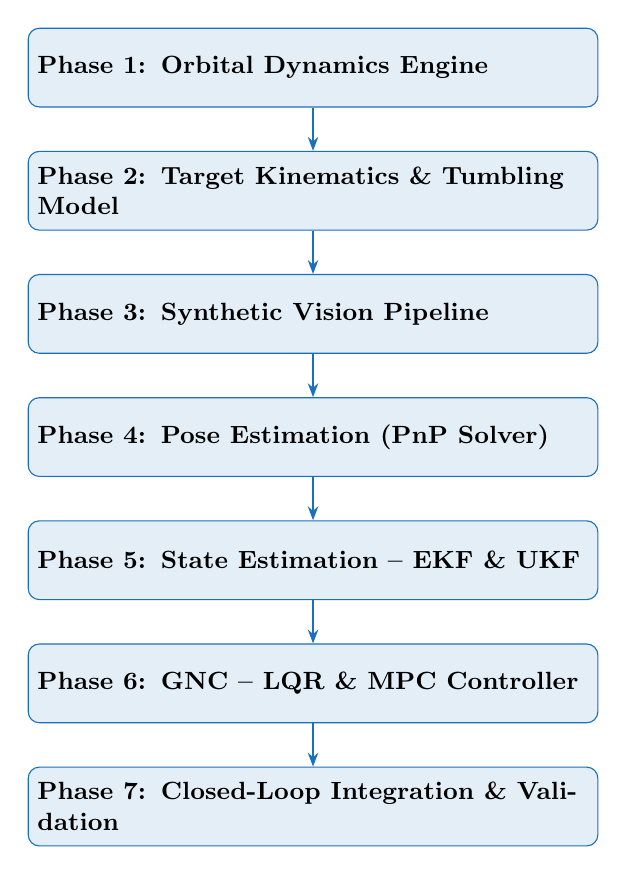
\begin{tikzpicture}[
    node distance=0.55cm,
    phase/.style={
        rectangle, rounded corners=4pt,
        draw=phaseblue, fill=phaseblue!12,
        text width=7cm, minimum height=1.0cm,
        align=left, font=\small\bfseries
    },
    arrow/.style={-{Stealth[length=5pt]}, thick, color=phaseblue}
]
\node[phase] (p1) {\textbf{Phase 1:} Orbital Dynamics Engine};
\node[phase, below=of p1] (p2) {\textbf{Phase 2:} Target Kinematics \& Tumbling Model};
\node[phase, below=of p2] (p3) {\textbf{Phase 3:} Synthetic Vision Pipeline};
\node[phase, below=of p3] (p4) {\textbf{Phase 4:} Pose Estimation (PnP Solver)};
\node[phase, below=of p4] (p5) {\textbf{Phase 5:} State Estimation -- EKF \& UKF};
\node[phase, below=of p5] (p6) {\textbf{Phase 6:} GNC -- LQR \& MPC Controller};
\node[phase, below=of p6] (p7) {\textbf{Phase 7:} Closed-Loop Integration \& Validation};

\draw[arrow] (p1) -- (p2);
\draw[arrow] (p2) -- (p3);
\draw[arrow] (p3) -- (p4);
\draw[arrow] (p4) -- (p5);
\draw[arrow] (p5) -- (p6);
\draw[arrow] (p6) -- (p7);
\end{tikzpicture}
\end{center}

\subsection*{Phase Deliverable Summary}

\begin{longtable}{@{}lp{5.5cm}p{5.5cm}@{}}
\toprule
\textbf{Phase} & \textbf{Core Deliverable} & \textbf{Key Algorithms / Assets} \\
\midrule
1 & HCW + YA propagator, J2 model & HCW ODEs, Yamanaka-Ankersen STM \\
2 & Rigid-body attitude simulator & Euler's rotation equations, quaternion kinematics \\
3 & Synthetic camera + renderer & Pinhole model, OpenCV, Blender API \\
4 & 6-DOF pose from images & EPnP, ORB/ArUco feature extraction \\
5 & EKF \& UKF state estimator & Jacobian propagation, sigma-point transform \\
6 & LQR + MPC thrust planner & DARE solver, OSQP / CasADi \\
7 & Full integrated simulator + Monte Carlo & GoogleTest, Matplotlib 3D, statistical analysis \\
\bottomrule
\end{longtable}

%% ============================================================
\section{Phase 1 -- Orbital Dynamics Engine}

\begin{phasebox}{Phase 1: Orbital Dynamics Engine}
\textbf{Goal:} Build the numerical backbone that propagates the relative
position and velocity of the chaser with respect to the tumbling target in
the Local-Vertical Local-Horizontal (LVLH) frame.\\[0.5em]
\textbf{Outputs:} \texttt{dynamics/hcw.py}, \texttt{dynamics/ya\_stm.cpp},
\texttt{dynamics/j2\_perturb.cpp}
\end{phasebox}

\subsection{Reference Frames}

\begin{itemize}[leftmargin=2em]
    \item \textbf{ECI (Earth-Centred Inertial):} Origin at Earth's CoM, axes
          fixed to distant stars. Used for absolute orbit propagation.
    \item \textbf{LVLH:} Origin at the chief (target) satellite. $\hat{x}$
          along the radial direction, $\hat{z}$ along orbit normal,
          $\hat{y} = \hat{z} \times \hat{x}$ (along-track).
\end{itemize}

\subsection{Hill--Clohessy--Wiltshire (HCW) Equations}

For a chaser in a \emph{near-circular} orbit about a chief, the linearised
relative equations of motion in the LVLH frame are:

\begin{formulabox}[title=HCW Equations of Relative Motion]
\begin{align}
\ddot{x} - 2n\dot{y} - 3n^2 x &= f_x \label{eq:hcw_x}\\
\ddot{y} + 2n\dot{x}           &= f_y \label{eq:hcw_y}\\
\ddot{z} + n^2 z               &= f_z \label{eq:hcw_z}
\end{align}
where $n = \sqrt{\mu / a^3}$ is the mean motion of the chief orbit,
$\mu = 3.986004418 \times 10^{14}\ \mathrm{m^3\,s^{-2}}$ is Earth's
gravitational parameter, $a$ is the chief semi-major axis, and
$f_x, f_y, f_z$ are the control accelerations per unit mass on the chaser.
\end{formulabox}

The HCW state vector is $\vx_{\HCW} = [x,\, y,\, z,\, \dot{x},\, \dot{y},\,
\dot{z}]^\top \in \mathbb{R}^6$. The system matrix is:

\begin{equation}
\mA_{\HCW} =
\begin{pmatrix}
0 & 0 & 0 & 1 & 0 & 0 \\
0 & 0 & 0 & 0 & 1 & 0 \\
0 & 0 & 0 & 0 & 0 & 1 \\
3n^2 & 0 & 0 & 0 & 2n & 0 \\
0 & 0 & 0 & -2n & 0 & 0 \\
0 & 0 & -n^2 & 0 & 0 & 0
\end{pmatrix}, \qquad
\mB = \begin{pmatrix} \mathbf{0}_{3\times3} \\ \mathbf{I}_{3\times3} \end{pmatrix}
\end{equation}

\subsection{Yamanaka--Ankersen State Transition Matrix (YA-STM)}

For \emph{elliptic} orbits (eccentricity $e > 0$), the HCW model loses
accuracy. The Yamanaka-Ankersen STM provides an analytic solution valid
for any eccentricity:

\begin{formulabox}[title=YA State Transition Matrix]
\begin{equation}
\vx(f) = \bm{\Phi}(f, f_0)\, \vx(f_0)
\end{equation}

where $f$ is true anomaly and the STM $\bm{\Phi}(f, f_0) \in
\mathbb{R}^{6\times6}$ is constructed from the fundamental solution
matrix:
\begin{equation}
\bm{\Phi}(f,f_0) = \mathbf{M}(f)\,\mathbf{M}^{-1}(f_0)
\end{equation}
with $\rho = 1 + e\cos f$, $s = \rho \sin f$, $c = \rho \cos f$,
and $J = \int_{f_0}^{f} \frac{df'}{\rho^2(f')}$ (computed numerically).

The columns of $\mathbf{M}(f)$ are the six particular solutions of the
homogeneous relative motion equations in the eccentric orbit case.
\end{formulabox}

\subsection{J\textsubscript{2} Perturbation}

The dominant gravitational perturbation for LEO is the oblateness of Earth
($J_2 = 1.08263 \times 10^{-3}$). Its acceleration in ECI coordinates is:

\begin{formulabox}[title=$J_2$ Perturbing Acceleration]
\begin{equation}
\mathbf{a}_{J_2} = \frac{3\mu J_2 R_E^2}{2r^5}
\begin{pmatrix}
x\!\left(5\frac{z^2}{r^2} - 1\right)\\[4pt]
y\!\left(5\frac{z^2}{r^2} - 1\right)\\[4pt]
z\!\left(5\frac{z^2}{r^2} - 3\right)
\end{pmatrix}
\end{equation}
where $R_E = 6{,}371\ \mathrm{km}$, $r = \|\vr\|$.
\end{formulabox}

\subsection{Phase 1 Asset Summary}
\begin{assetbox}[title=Phase 1 Assets]
\begin{itemize}[leftmargin=1.5em, itemsep=2pt]
    \item \textbf{Libraries:} NumPy, SciPy (\texttt{solve\_ivp} RK45/DOP853),
          Eigen3 (C++)
    \item \textbf{Constants:} $\mu$, $J_2$, $R_E$, $\omega_E$ (Earth rotation rate)
    \item \textbf{Test:} HCW drift-free periodic orbit verification,
          energy conservation check
    \item \textbf{Output:} Time-series $[\vr(t), \vv(t)]$ in LVLH frame
\end{itemize}
\end{assetbox}

%% ============================================================
\section{Phase 2 -- Target Kinematics \& Tumbling Model}

\begin{phasebox}{Phase 2: Target Kinematics \& Tumbling}
\textbf{Goal:} Simulate the uncontrolled attitude dynamics of a rigid
debris body (e.g., an upper rocket stage) including torque-free tumbling.\\[0.5em]
\textbf{Outputs:} \texttt{target/attitude.py}, \texttt{target/rigid\_body.cpp}
\end{phasebox}

\subsection{Rigid-Body Rotational Dynamics -- Euler's Equations}

\begin{formulabox}[title=Euler's Equations (Body Frame)]
\begin{align}
I_1 \dot{\omega}_1 &= (I_2 - I_3)\,\omega_2\,\omega_3 + \tau_1 \\
I_2 \dot{\omega}_2 &= (I_3 - I_1)\,\omega_3\,\omega_1 + \tau_2 \\
I_3 \dot{\omega}_3 &= (I_1 - I_2)\,\omega_1\,\omega_2 + \tau_3
\end{align}
For torque-free tumbling debris, $\bm{\tau} = \mathbf{0}$.
$\mathbf{I} = \mathrm{diag}(I_1, I_2, I_3)$ is the principal-axis
inertia tensor.
\end{formulabox}

\subsection{Attitude Representation -- Unit Quaternion}

A unit quaternion $\vq = [q_0,\, \mathbf{q}_v]^\top$ with $q_0 \in
\mathbb{R}$ and $\mathbf{q}_v \in \mathbb{R}^3$, $\|\vq\| = 1$,
parameterises the rotation matrix as:

\begin{equation}
\mathbf{C}(\vq) = (q_0^2 - \|\mathbf{q}_v\|^2)\mathbf{I}_3
+ 2\mathbf{q}_v\mathbf{q}_v^\top + 2q_0\,[\mathbf{q}_v]_\times
\end{equation}

where $[\cdot]_\times$ is the skew-symmetric cross-product matrix.

\begin{formulabox}[title=Quaternion Kinematics]
\begin{equation}
\dot{\vq} = \frac{1}{2} \bm{\Xi}(\vq)\, \vw, \qquad
\bm{\Xi}(\vq) =
\begin{pmatrix}
-\mathbf{q}_v^\top \\
q_0 \mathbf{I}_3 + [\mathbf{q}_v]_\times
\end{pmatrix} \in \mathbb{R}^{4\times3}
\end{equation}
\end{formulabox}

\noindent The combined attitude-rate state is $\vx_{\mathrm{att}} =
[\vq^\top,\, \vw^\top]^\top \in \mathbb{R}^7$.

\subsection{Phase 2 Asset Summary}
\begin{assetbox}[title=Phase 2 Assets]
\begin{itemize}[leftmargin=1.5em, itemsep=2pt]
    \item Inertia tensor $\mathbf{I}$ for a representative cylindrical debris
          body (e.g., Ariane upper stage geometry)
    \item Quaternion normalisation constraint enforcement
    \item Simulation of Euler angles, Polhode trajectory (torque-free)
    \item Libraries: \texttt{scipy.integrate}, Eigen3, \texttt{pyquaternion}
\end{itemize}
\end{assetbox}

%% ============================================================
\section{Phase 3 -- Synthetic Vision Pipeline}

\begin{phasebox}{Phase 3: Synthetic Vision Pipeline}
\textbf{Goal:} Generate realistic monocular grayscale/RGB images of the
tumbling target at each simulation time step, with controllable camera
noise, sensor blur, and lighting.\\[0.5em]
\textbf{Outputs:} \texttt{vision/camera.py}, \texttt{vision/renderer.py},
\texttt{vision/feature\_extractor.py}
\end{phasebox}

\subsection{Pinhole Camera Model}

\begin{formulabox}[title=Pinhole Projection]
\begin{equation}
\lambda \begin{pmatrix} u \\ v \\ 1 \end{pmatrix}
= \mathbf{K}\, [\mathbf{R}_c \mid \mathbf{t}_c]\,
\begin{pmatrix} X \\ Y \\ Z \\ 1 \end{pmatrix}
\end{equation}

Camera intrinsic matrix:
\begin{equation}
\mathbf{K} =
\begin{pmatrix}
f_x & 0   & c_x \\
0   & f_y & c_y \\
0   & 0   & 1
\end{pmatrix}
\end{equation}
where $f_x = f/d_x$, $f_y = f/d_y$ are the focal lengths in pixels,
$(c_x, c_y)$ is the principal point, and $\lambda$ is the depth scale
factor. $(\mathbf{R}_c, \mathbf{t}_c)$ are the camera extrinsic rotation
and translation.
\end{formulabox}

\subsection{Image Noise Model}

Each synthesised pixel intensity $I(u,v)$ is corrupted by additive white
Gaussian noise (AWGN) and a Poisson shot noise term:

\begin{equation}
\tilde{I}(u,v) = I(u,v) + \mathcal{N}(0, \sigma_{\mathrm{read}}^2)
+ \mathrm{Poisson}(I(u,v)/g)
\end{equation}

where $g$ is the sensor gain factor. Default parameters: $\sigma_{\mathrm{read}}
= 2\ \mathrm{DN}$, $g = 4\ \mathrm{e^-/DN}$.

\subsection{Feature Extraction Pipeline}

\begin{center}
\begin{tabular}{lll}
\toprule
\textbf{Method} & \textbf{Use Case} & \textbf{Library} \\
\midrule
ArUco Markers   & Known-target simulation / ground truth & \texttt{cv2.aruco} \\
ORB             & Textured surfaces, real-imagery testing & \texttt{cv2.ORB} \\
Keypoint NN     & Deep learning pose estimation (Phase 4+) & PyTorch \\
\bottomrule
\end{tabular}
\end{center}

\subsection{Phase 3 Asset Summary}
\begin{assetbox}[title=Phase 3 Assets]
\begin{itemize}[leftmargin=1.5em, itemsep=2pt]
    \item \textbf{3D Mesh:} Blender `.obj` model of representative debris
          (Ariane 44L upper stage, or custom cylinder)
    \item \textbf{Renderer:} Blender Python API (\texttt{bpy}) or
          PyRenderer / ModernGL for real-time frames
    \item \textbf{Calibration:} Synthetic camera with $f = 50\ \mathrm{mm}$,
          $1024 \times 1024$ px, $\sigma_{\mathrm{px}} = 2\ \mathrm{px}$ noise
    \item \textbf{Dataset:} Generate $> 10{,}000$ labelled pose-image pairs
          for NN training (optional Phase 4 extension)
\end{itemize}
\end{assetbox}

%% ============================================================
\section{Phase 4 -- Pose Estimation (PnP Solver)}

\begin{phasebox}{Phase 4: Visual Pose Estimation}
\textbf{Goal:} From a set of 2D image keypoint correspondences to known
3D object body-frame points, recover the 6-DOF relative pose
$(\mathbf{R}, \mathbf{t})$ of the target in the camera frame.\\[0.5em]
\textbf{Outputs:} \texttt{estimation/pnp\_solver.py},
\texttt{estimation/epnp.cpp}
\end{phasebox}

\subsection{The Perspective-$n$-Point Problem}

Given $n$ correspondences $\{(\mathbf{p}_i, \mathbf{u}_i)\}_{i=1}^n$
where $\mathbf{p}_i \in \mathbb{R}^3$ are body-frame 3D control points
and $\mathbf{u}_i = (u_i, v_i)$ are image-plane pixel coordinates, find
$(\mathbf{R}, \mathbf{t})$ minimising the reprojection error:

\begin{formulabox}[title=PnP Reprojection Objective]
\begin{equation}
\min_{\mathbf{R} \in SO(3),\, \mathbf{t} \in \mathbb{R}^3}
\sum_{i=1}^{n}
\left\|
\mathbf{u}_i -
\pi\!\left(\mathbf{K}\left(\mathbf{R}\,\mathbf{p}_i + \mathbf{t}\right)\right)
\right\|^2
\end{equation}
where the projection $\pi\!\left([X,Y,Z]^\top\right) = [X/Z,\, Y/Z]^\top$.
\end{formulabox}

\subsection{EPnP Algorithm (Efficient PnP)}

EPnP (Lepetit et al., 2009) expresses the $n$ 3D points as weighted
combinations of 4 \emph{control points} $\mathbf{c}_j$:

\begin{equation}
\mathbf{p}_i = \sum_{j=1}^{4} \alpha_{ij}\, \mathbf{c}_j, \qquad
\sum_{j=1}^{4} \alpha_{ij} = 1
\end{equation}

This reduces the PnP problem to solving a $12 \times 12$ eigenvalue system,
achieving $O(n)$ complexity with sub-pixel accuracy.

\subsection{RANSAC Robustification}

To handle feature mismatches and image clutter, EPnP is embedded in a
RANSAC loop:

\begin{algorithm}[H]
\caption{RANSAC-EPnP Pose Estimation}
\begin{algorithmic}[1]
\For{$k = 1, \ldots, K_{\max}$}
    \State Sample 4 random correspondences
    \State Solve EPnP $\to (\mathbf{R}_k, \mathbf{t}_k)$
    \State Count inliers: $|\{i : \text{reproj error}_i < \epsilon\}|$
\EndFor
\State \textbf{Return} hypothesis with most inliers; refine with Levenberg-Marquardt
\end{algorithmic}
\end{algorithm}

\subsection{Phase 4 Asset Summary}
\begin{assetbox}[title=Phase 4 Assets]
\begin{itemize}[leftmargin=1.5em, itemsep=2pt]
    \item \texttt{cv2.solvePnP} with \texttt{SOLVEPNP\_EPNP} flag (baseline)
    \item Custom C++ EPnP for latency benchmarking
    \item Accuracy target: rotation error $< 1.5^\circ$,
          translation error $< 3\ \mathrm{cm}$ at $50\ \mathrm{m}$ range
    \item Ground-truth pose from Phase 1 \& 2 for error evaluation
\end{itemize}
\end{assetbox}

%% ============================================================
\section{Phase 5 -- State Estimation: EKF \& UKF}

\begin{phasebox}{Phase 5: Nonlinear State Estimation}
\textbf{Goal:} Fuse noisy PnP pose measurements with the orbital dynamics
model to reconstruct the full 12-state relative navigation state
$\vx = [\vr, \vv, \vq, \vw]^\top \in \mathbb{R}^{13}$ (with quaternion
unit-norm constraint).\\[0.5em]
\textbf{Outputs:} \texttt{estimation/ekf.py}, \texttt{estimation/ukf.py},
\texttt{estimation/ekf.cpp}
\end{phasebox}

\subsection{State \& Measurement Vectors}

\begin{equation}
\vx_k =
\underbrace{\begin{pmatrix} \vr_k \\ \vv_k \end{pmatrix}}_{\text{translational}}
\oplus
\underbrace{\begin{pmatrix} \vq_k \\ \vw_k \end{pmatrix}}_{\text{rotational}}
\in \mathbb{R}^{6} \oplus \mathbb{R}^{7}
\end{equation}

The measurement vector from the PnP solver:
$\mathbf{z}_k = [\hat{\vr}_k^\top,\, \hat{\vq}_k^\top]^\top \in \mathbb{R}^{7}$

\subsection{Extended Kalman Filter (EKF)}

\begin{formulabox}[title=EKF Predict--Update Cycle]
\textbf{Predict:}
\begin{align}
\hat{\vx}_{k|k-1} &= f(\hat{\vx}_{k-1|k-1}, \vcu_{k-1}) \\
\mP_{k|k-1}       &= \mF_{k-1}\,\mP_{k-1|k-1}\,\mF_{k-1}^\top + \mQ
\end{align}

\textbf{Update:}
\begin{align}
\mathbf{S}_k &= \mH_k\,\mP_{k|k-1}\,\mH_k^\top + \mR \\
\mK_k        &= \mP_{k|k-1}\,\mH_k^\top\,\mathbf{S}_k^{-1} \\
\hat{\vx}_{k|k} &= \hat{\vx}_{k|k-1} + \mK_k\!\left(\mathbf{z}_k - h(\hat{\vx}_{k|k-1})\right) \\
\mP_{k|k}    &= (\mathbf{I} - \mK_k \mH_k)\,\mP_{k|k-1}
\end{align}

Jacobians: $\mF_k = \left.\frac{\partial f}{\partial \vx}\right|_{\hat{\vx}_{k|k}}$,\quad
$\mH_k = \left.\frac{\partial h}{\partial \vx}\right|_{\hat{\vx}_{k|k-1}}$
\end{formulabox}

\subsection{Unscented Kalman Filter (UKF)}

The UKF avoids linearisation by propagating a set of $2L+1$ deterministically
chosen \emph{sigma points} through the nonlinear functions, where $L = \dim(\vx)$.

\begin{formulabox}[title=Merwe-Scaled Sigma Point Selection]
\begin{align}
\bm{\sigma}_0     &= \hat{\vx} \\
\bm{\sigma}_i     &= \hat{\vx} + \left(\sqrt{(L+\lambda)\mP}\right)_i, \quad i = 1,\ldots,L \\
\bm{\sigma}_{i+L} &= \hat{\vx} - \left(\sqrt{(L+\lambda)\mP}\right)_i, \quad i = 1,\ldots,L
\end{align}
Scaling: $\lambda = \alpha^2(L + \kappa) - L$ with $\alpha = 10^{-3}$,
$\kappa = 0$, $\beta = 2$ (Gaussian prior assumption).
\end{formulabox}

\subsection{Noise Covariance Matrices}

\begin{align}
\mQ &= \mathrm{diag}\!\left(\sigma_{\vr}^2\,\mathbf{I}_3,\;
       \sigma_{\vv}^2\,\mathbf{I}_3,\;
       \sigma_{q}^2\,\mathbf{I}_4,\;
       \sigma_{\omega}^2\,\mathbf{I}_3\right) \\[4pt]
\mR &= \mathrm{diag}\!\left(\sigma_{\mathrm{pos,meas}}^2\,\mathbf{I}_3,\;
       \sigma_{\mathrm{att,meas}}^2\,\mathbf{I}_4\right)
\end{align}

Typical LEO tuning values:
$\sigma_{\vr} = 0.01\ \mathrm{m}$,
$\sigma_{\vv} = 0.001\ \mathrm{m/s}$,
$\sigma_q = 10^{-4}$,
$\sigma_{\mathrm{pos,meas}} = 0.05\ \mathrm{m}$ (from PnP noise level).

\subsection{Phase 5 Asset Summary}
\begin{assetbox}[title=Phase 5 Assets]
\begin{itemize}[leftmargin=1.5em, itemsep=2pt]
    \item Python: \texttt{filterpy} library (EKF, UKF baseline)
    \item C++: Custom EKF with Eigen3 matrix operations
    \item Quaternion EKF: Multiplicative EKF (MEKF) to respect $SO(3)$ manifold
    \item Performance metric: 3-$\sigma$ consistency test (NIS/NEES)
\end{itemize}
\end{assetbox}

%% ============================================================
\section{Phase 6 -- GNC: Guidance, Navigation \& Control}

\begin{phasebox}{Phase 6: Closed-Loop Control}
\textbf{Goal:} Using the estimated state from Phase 5, compute an
optimal thrust sequence that drives the chaser to the desired hold-point
(e.g., $10\ \mathrm{m}$ stand-off) while minimising propellant consumption.\\[0.5em]
\textbf{Outputs:} \texttt{control/lqr.py}, \texttt{control/mpc.py}
\end{phasebox}

\subsection{Linear Quadratic Regulator (LQR)}

For the linearised HCW system $(\mA_{\HCW}, \mB)$, the LQR gain matrix
$\mK_{\mathrm{LQR}}$ minimises the infinite-horizon cost:

\begin{formulabox}[title=LQR Cost Function]
\begin{equation}
J_{\mathrm{LQR}} = \int_0^\infty
\left[\vx^\top \mathbf{Q}_c\, \vx + \vcu^\top \mathbf{R}_c\, \vcu\right] dt
\end{equation}
Optimal gain: $\mK_{\mathrm{LQR}} = \mathbf{R}_c^{-1} \mB^\top \mathbf{P}^*$\\
where $\mathbf{P}^*$ solves the Algebraic Riccati Equation (ARE):
\begin{equation}
\mA^\top \mathbf{P}^* + \mathbf{P}^* \mA
- \mathbf{P}^* \mB \mathbf{R}_c^{-1} \mB^\top \mathbf{P}^* + \mathbf{Q}_c = \mathbf{0}
\end{equation}
\end{formulabox}

Control law: $\vcu^*(t) = -\mK_{\mathrm{LQR}}\, \vx(t)$.

\subsection{Discrete-Time Model Predictive Control (MPC)}

MPC optimises a finite receding-horizon trajectory subject to constraints.
At each time step $k$, solve:

\begin{formulabox}[title=MPC Optimisation Problem]
\begin{equation}
\min_{\vcu_0, \ldots, \vcu_{N-1}}
\sum_{j=0}^{N-1}\!\left[\vx_j^\top \mathbf{Q}_c\, \vx_j
+ \vcu_j^\top \mathbf{R}_c\, \vcu_j\right]
+ \vx_N^\top \mathbf{P}^* \vx_N
\end{equation}
\textbf{Subject to:}
\begin{align}
\vx_{j+1}     &= \mA_d\, \vx_j + \mB_d\, \vcu_j \quad (\text{discrete HCW}) \\
\|\vcu_j\|_2   &\leq u_{\max}                       \quad (\text{thrust limit}) \\
\sum_j \|\vcu_j\|_1 &\leq \Deltav_{\mathrm{budget}}     \quad (\text{fuel budget})
\end{align}
\end{formulabox}

The problem is a quadratic program (QP); solved with OSQP at $\sim 100$
Hz onboard control loop frequency.

Discretisation ($T_s$ = sample period):
\begin{equation}
\mA_d = e^{\mA_{\HCW} T_s}, \qquad
\mB_d = \left(\int_0^{T_s} e^{\mA_{\HCW}\tau} d\tau\right) \mB
\end{equation}

\subsection{$\Delta v$ Budget Analysis}

Total propellant consumed during a rendezvous sequence of $M$ manoeuvres:
\begin{equation}
\Deltav_{\mathrm{total}} = \sum_{k=1}^{M} \|\Delta\mathbf{v}_k\|_2, \qquad
m_{\mathrm{prop}} = m_0\!\left(1 - e^{-\Deltav_{\mathrm{total}}/(\Isp\, g_0)}\right)
\end{equation}

\subsection{Phase 6 Asset Summary}
\begin{assetbox}[title=Phase 6 Assets]
\begin{itemize}[leftmargin=1.5em, itemsep=2pt]
    \item \textbf{LQR:} \texttt{scipy.linalg.solve\_continuous\_are} /
          \texttt{control.lqr}
    \item \textbf{MPC:} \texttt{osqp-python}, \texttt{CasADi} (for nonlinear MPC extension)
    \item \textbf{Constraints:} $u_{\max} = 1\ \mathrm{N}$ (cold-gas thruster budget),
          $\Deltav \leq 20\ \mathrm{m/s}$ total
    \item \textbf{Benchmark:} MPC vs PD controller $\Deltav$ comparison
\end{itemize}
\end{assetbox}

%% ============================================================
\section{Phase 7 -- Closed-Loop Integration \& Validation}

\begin{phasebox}{Phase 7: System Integration \& Monte Carlo Validation}
\textbf{Goal:} Integrate all six prior modules into a single simulation
loop and perform statistical validation through Monte Carlo analysis.\\[0.5em]
\textbf{Outputs:} \texttt{sim/main\_loop.py}, \texttt{tests/}, plots,
final benchmark table
\end{phasebox}

\subsection{Closed-Loop Simulation Block Diagram}

At each time step $k$ of the simulation:
\begin{enumerate}[leftmargin=2em, itemsep=3pt]
    \item \textbf{Propagate:} Phase 1 $\rightarrow$ update $[\vr_k, \vv_k]_{\LVLH}$
    \item \textbf{Attitude:} Phase 2 $\rightarrow$ update $[\vq_k, \vw_k]$ of target
    \item \textbf{Render:} Phase 3 $\rightarrow$ generate synthetic camera frame $I_k$
    \item \textbf{Detect:} Phase 3 $\rightarrow$ extract keypoints/features from $I_k$
    \item \textbf{PnP:} Phase 4 $\rightarrow$ recover noisy pose measurement $\mathbf{z}_k$
    \item \textbf{Filter:} Phase 5 $\rightarrow$ EKF/UKF update $\to \hat{\vx}_k$
    \item \textbf{Control:} Phase 6 $\rightarrow$ MPC solve $\to \vcu_k^*$
    \item \textbf{Apply:} Thrust $\vcu_k^*$ feeds back into Phase 1 as $f_x, f_y, f_z$
\end{enumerate}

\subsection{Monte Carlo Performance Metrics}

Run $N_{\mathrm{MC}} = 500$ trials with randomly sampled:
\begin{itemize}[leftmargin=2em]
    \item Initial relative position: $\vr_0 \sim \mathcal{U}([50, 200]\ \mathrm{m})$
    \item Camera pixel noise: $\sigma_{\mathrm{px}} \sim \mathcal{U}(0.5, 3.0)\ \mathrm{px}$
    \item Target tumble rate: $\vw_0 \sim \mathcal{U}(0.5, 5.0)\ \mathrm{deg/s}$
\end{itemize}

\begin{center}
\begin{tabular}{llll}
\toprule
\textbf{Metric} & \textbf{Definition} & \textbf{Target} & \textbf{Units} \\
\midrule
Position Error & $\|\hat{\vr} - \vr\|_2$ & $< 0.05$ & m \\
Velocity Error & $\|\hat{\vv} - \vv\|_2$ & $< 0.01$ & m/s \\
Attitude Error & $2\arccos(|\hat{q}_0 q_0 + \hat{\mathbf{q}}_v \cdot \mathbf{q}_v|)$ & $< 1.2$ & deg \\
$\Deltav$ Consumed & $\sum\|\Delta\mathbf{v}\|$ (MPC vs LQR) & 14\% saving & m/s \\
PnP Latency & Time per frame & $< 10$ & ms \\
Filter NIS & Normalised innovation & $\chi^2_{n_z,95\%}$ & --- \\
\bottomrule
\end{tabular}
\end{center}

\subsection{Unit Test Suite}
\begin{itemize}[leftmargin=2em, itemsep=2pt]
    \item HCW drift-free orbit: 5-orbit propagation without divergence
    \item EKF consistency: NIS $\chi^2$ test at 95\% confidence
    \item PnP accuracy: sub-pixel reprojection error on synthetic data
    \item MPC feasibility: QP solved in $< 10\ \mathrm{ms}$, constraints satisfied
\end{itemize}

%% ============================================================
\section{Complete Asset \& Dependency Register}

\begin{longtable}{@{}llp{7cm}@{}}
\toprule
\textbf{Category} & \textbf{Tool / Library} & \textbf{Purpose} \\
\midrule
\endhead
\multicolumn{3}{c}{\textit{--- Core Languages ---}} \\
Language & Python 3.11 & Simulation, data pipeline, visualisation \\
Language & C++17       & EKF/UKF core, EPnP, performance-critical code \\
Build    & CMake 3.25  & C++ build system \\
\midrule
\multicolumn{3}{c}{\textit{--- Numerical / Scientific ---}} \\
NumPy & 1.26 & Array ops, linear algebra \\
SciPy & 1.12 & ODE integration (RK45, DOPRI853), ARE solver \\
Eigen3 & 3.4 & C++ matrix library \\
Matplotlib & 3.8 & 2D/3D plotting, Monte Carlo histograms \\
\midrule
\multicolumn{3}{c}{\textit{--- Computer Vision ---}} \\
OpenCV & 4.9 & Camera model, PnP, ORB/ArUco, RANSAC \\
Blender Python API & 4.x & 3D mesh rendering (offline frames) \\
PyTorch & 2.2 & Keypoint NN (optional Phase 4 extension) \\
\midrule
\multicolumn{3}{c}{\textit{--- Estimation \& Control ---}} \\
filterpy & 1.4 & EKF, UKF reference implementation \\
python-control & 0.9 & LQR, ARE, Bode/root-locus analysis \\
CasADi & 3.6 & Symbolic differentiation, NLP/MPC formulation \\
OSQP & 0.6 & Fast QP solver for MPC \\
\midrule
\multicolumn{3}{c}{\textit{--- Astrodynamics ---}} \\
Astropy & 6.0 & Time conversions, coordinate frames \\
Poliastro & 0.17 & Orbit propagation baseline comparison \\
\midrule
\multicolumn{3}{c}{\textit{--- Testing \& CI ---}} \\
GoogleTest & 1.14 & C++ unit tests \\
pytest & 8.0 & Python unit/integration tests \\
GitHub Actions & --- & CI pipeline (build, test, lint) \\
\bottomrule
\end{longtable}

%% ============================================================
\section{Key Mathematical Symbols Reference}

\begin{longtable}{@{}lp{9cm}l@{}}
\toprule
\textbf{Symbol} & \textbf{Definition} & \textbf{Units} \\
\midrule
\endhead
$n$ & Mean orbital motion of chief, $n = \sqrt{\mu/a^3}$ & rad/s \\
$\mu$ & Earth gravitational parameter & m$^3$ s$^{-2}$ \\
$a$ & Chief orbit semi-major axis & m \\
$e$ & Orbital eccentricity & --- \\
$J_2$ & Earth oblateness coefficient & --- \\
$\vr$ & Relative position in LVLH & m \\
$\vv$ & Relative velocity in LVLH & m/s \\
$\vq$ & Unit quaternion (target attitude) & --- \\
$\vw$ & Angular velocity (target body frame) & rad/s \\
$\mathbf{I}$ & Principal inertia tensor & kg$\cdot$m$^2$ \\
$\mathbf{K}$ & Camera intrinsic matrix & px \\
$\mathbf{R}_c, \mathbf{t}_c$ & Camera extrinsic rotation \& translation & ---/m \\
$\mP$ & State error covariance matrix & (state units)$^2$ \\
$\mQ$ & Process noise covariance & (state units)$^2$ \\
$\mR$ & Measurement noise covariance & (meas units)$^2$ \\
$\mK$ & Kalman gain matrix & --- \\
$\mathbf{Q}_c, \mathbf{R}_c$ & LQR/MPC cost weight matrices & --- \\
$\Deltav$ & Delta-velocity manoeuvre magnitude & m/s \\
$\Isp$ & Engine specific impulse & s \\
$N$ & MPC prediction horizon & steps \\
$T_s$ & Discrete control sample period & s \\
\bottomrule
\end{longtable}

%% ============================================================
\section{Repository Structure}

\begin{verbatim}
vision-satellite-rendezvous/
|-- config/
|   |-- orbit_params.yaml          # Chief orbit, simulation duration
|   |-- camera_params.yaml         # Intrinsics, noise parameters
|   `-- control_params.yaml        # MPC horizon, LQR weights
|-- dynamics/
|   |-- hcw.py                     # Phase 1: HCW propagator
|   |-- ya_stm.cpp                 # Phase 1: YA state-transition matrix
|   `-- j2_perturb.cpp             # Phase 1: J2 acceleration
|-- target/
|   |-- attitude.py                # Phase 2: Euler + quaternion kinematics
|   `-- rigid_body.cpp             # Phase 2: C++ rigid-body integrator
|-- vision/
|   |-- camera.py                  # Phase 3: Pinhole model, distortion
|   |-- renderer.py                # Phase 3: Blender/OpenCV renderer
|   `-- feature_extractor.py       # Phase 3: ORB, ArUco, keypoint NN
|-- estimation/
|   |-- pnp_solver.py              # Phase 4: EPnP + RANSAC wrapper
|   |-- epnp.cpp                   # Phase 4: C++ EPnP core
|   |-- ekf.py                     # Phase 5: EKF (translational + MEKF)
|   `-- ukf.py                     # Phase 5: UKF with sigma points
|-- control/
|   |-- lqr.py                     # Phase 6: LQR design (ARE solver)
|   `-- mpc.py                     # Phase 6: OSQP-based MPC
|-- sim/
|   `-- main_loop.py               # Phase 7: Closed-loop simulation entry
|-- tests/
|   |-- test_hcw.cpp               # GoogleTest: HCW orbit conservation
|   |-- test_ekf.py                # pytest: EKF NIS consistency
|   `-- test_pnp.py                # pytest: PnP reprojection accuracy
|-- notebooks/
|   `-- phase_demo.ipynb           # Jupyter notebooks per phase
|-- CMakeLists.txt
|-- requirements.txt
`-- README.md
\end{verbatim}

%% ============================================================
\section{Expected Results \& Publication-Grade Benchmarks}

\begin{center}
\renewcommand{\arraystretch}{1.3}
\begin{tabular}{llll}
\toprule
\textbf{Result} & \textbf{Phase} & \textbf{Expected Value} & \textbf{Comparison} \\
\midrule
Steady-state position error & 5 & $< 0.05$ m & EKF vs UKF \\
Attitude estimation error   & 5 & $< 1.2^\circ$ & MEKF consistency \\
PnP rotation error          & 4 & $< 1.5^\circ$ & ORB vs ArUco \\
MPC $\Deltav$ saving            & 6 & $\approx 14\%$ & MPC vs PD \\
MPC solve time              & 6 & $< 10$ ms     & OSQP hot-start \\
Monte Carlo pass rate       & 7 & $> 95\%$      & 500 trials \\
\bottomrule
\end{tabular}
\end{center}

%% ============================================================
\section{Conclusion \& Next Steps}

This blueprint defines a complete, executable path from first principles
to a publication-quality closed-loop space rendezvous simulator.
Each of the seven phases is independently testable and produces a
concrete artefact. The mathematical formulations are grounded in
established aerospace literature (HCW, YA, EPnP, MEKF, MPC-OSQP)
while the implementation stack (C++17 + Python 3.11, OpenCV, Eigen3,
CasADi) reflects real-world flight-software practice.

\textbf{Immediate next steps after this document:}
\begin{enumerate}[leftmargin=2em]
    \item Set up GitHub repository and CI skeleton
    \item Implement and test Phase 1 (HCW + J2) with unit test coverage
    \item Validate against Poliastro reference propagator
    \item Begin Phase 2 attitude integrator in parallel
\end{enumerate}

\vspace{1em}
\hrule
\vspace{0.5em}
\begin{center}
\small\textcolor{darkgray}{
Vision-Based Satellite Rendezvous Simulator -- Blueprint v1.0\\
Bishwaswarup Nayak $\cdot$ August 2026}
\end{center}

\end{document}
